%%%%%%%%%%%%%%%%%%%%%%%%%%%%%%%%%%%%%%%%%%%%%%%%%%%%%%%%%%%
% --------------------------------------------------------
% Tau
% LaTeX Template
% Version 2.4.3 (01/09/2024)
%
% Author: 
% Guillermo Jimenez (memo.notess1@gmail.com)
% 
% License:
% Creative Commons CC BY 4.0
% --------------------------------------------------------
%%%%%%%%%%%%%%%%%%%%%%%%%%%%%%%%%%%%%%%%%%%%%%%%%%%%%%%%%%%

\documentclass[9pt,a4paper,twoside]{tau-class/tau}
\usepackage[english]{babel}

%----------------------------------------------------------
% TITLE
%----------------------------------------------------------

\journalname{Aprenentatge Computacional}
%% TODO: Optional, you can set a fancier title if you like
\title{Sign Language ASL Recognition using Bag of Visual Words and Support Vector Machines}

%----------------------------------------------------------
% AUTHORS, AFFILIATIONS AND PROFESSOR
%----------------------------------------------------------

%% TODO: Set your names here
\author[a]{Samuel Ortega Cuadra}
\author[b]{Laia Alexandra Sjöberg Cerezo}

%----------------------------------------------------------

\affil[a]{1669776}
\affil[b]{1667894}


%----------------------------------------------------------
% FOOTER INFORMATION
%----------------------------------------------------------

\institution{Universitat Autònoma de Barcelona}
\footinfo{Class Project}
\theday{December 10, 2024}
\leadauthor{Group XX} 		%% TODO: Set your group ID here
\course{Aprenentatge Computacional}

%----------------------------------------------------------
% ABSTRACT AND KEYWORDS
%----------------------------------------------------------

\begin{abstract}    
	%% TODO: Change this default abstract into something nice that describes your work.
	%% Keep it below 300 words.
    This project focuses on developing a system for recognizing American Sign Language (ASL) alphabet and numbers. The proposed approach combines image preprocessing, feature extraction, and prediction models to accurately classify hand gestures. The dataset consists of images of hands representing ASL letters and numbers, which are processed by isolating the hand region, converting it in grayscale and applying a mask for feature extraction. Dense SIFT and a Bag of Words model are used to create feature representations, and a Support Vector Machine (SVM) classifier is trained and optimized through grid search for maximum accuracy.
    
    The finished system can recognize hands by retrieving frames from video input, and translating ASL gesture sequences into coherent text. 
    
    This work lays a foundation for future developments in sign language recognition and improving accessibility for the deaf community by providing a tool for real-time translation of sign language to text.
\end{abstract}

%----------------------------------------------------------

%% TODO: Set appropriate keywords for your report.
%\keywords{a, b, c, d}

%----------------------------------------------------------

\begin{document}
	%% Do NOT change any of this. Line numbers should be kept.
    \maketitle 
    \thispagestyle{firststyle} \tauabstract 
    \tableofcontents
    \linenumbers 
    
%----------------------------------------------------------

\section{Introduction}

    \taustart{T}his document presents the development of a system for recognizing American Sign Language (ASL) alphabet and numbers. It outlines the steps taken to achieve this goal, from the \textbf{dataset collection} and preprocessing to the implementation of a \textbf{Bag of Visual Words} to help builiding a \textbf{SVM model} for classification. The system is then extended to \textbf{process videos}, extract frames, identify ASL symbols, and \textbf{reconstruct} the words being spelled.
\section{Finding The Dataset}

	When looking for a good ASL dataset, we found the \href{https://www.kaggle.com/datasets/ayuraj/asl-dataset}{American Sign Language Dataset} dataset on Kaggle. This dataset contains 2515 images of 400x400 pixels, each showing a hand making an ASL letter or number. The dataset is divided into 36 folders, one for each letter of the alphabet and one for each of the numbers from 0 to 9. The images are in JPEG format and have a black background with a white hand. The dataset is well-organized and easy to use, making it a good choice for our project.

    \subsection{Dataset Preprocessing}

    The preprocessing of the dataset invloves the following steps: 
    \begin{enumerate}
        \item \textbf{Dataset Organization}: The dataset is organized into folders, one for each letter of the alphabet and one for each number from 0 to 9. Each folder contains 65 to 70 images of hands making the corresponding ASL symbol. A \textit{categories} dictionary was created to map each label to its corresponding folder name. The filenames of all images were collected and combined with their respective category labels to construct a DataFrame.
        \item \textbf{Shuffiling the Dataset}: To avoid any bias in the training and testing data, the dataset was shuffled. This ensures that the data is randomly distributed and that the model will not be trained on any specific order of images.
        \item \textbf{Image Loading}: Each image was loaded from its respective path and converted into a NumPy array. Providing a new variable with a structured representation of pixels called \textit{pixel\_ data}.
        \item \textbf{Grayscale conversion}: The images were converted to grayscale to reduce the complexity of the model and improve training speed.
    \end{enumerate}
    \begin{figure}[H]
		\centering
		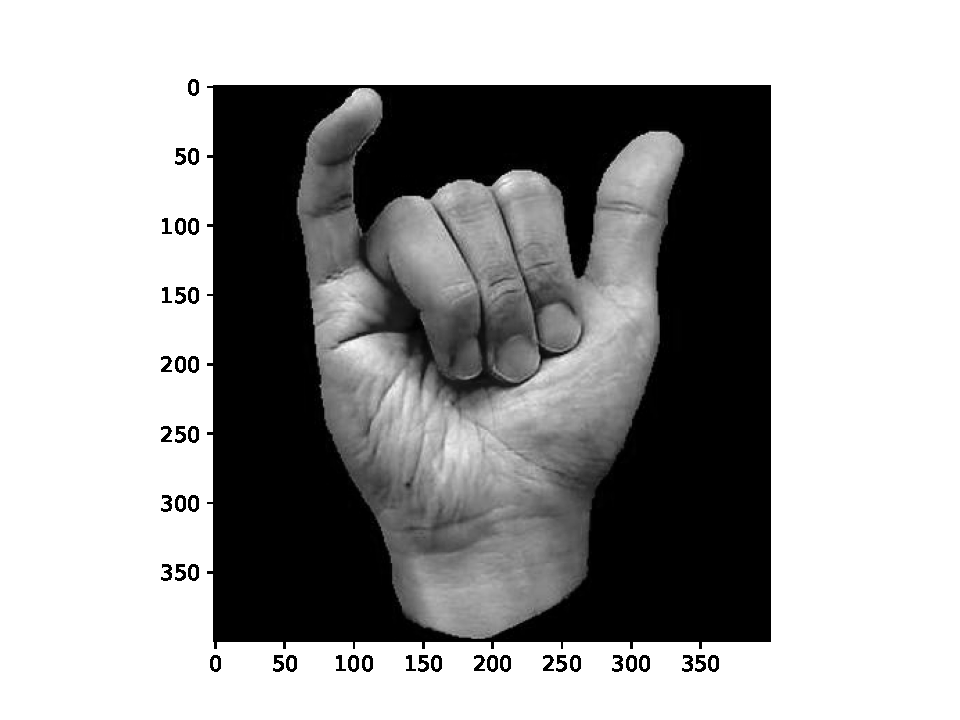
\includegraphics[width=0.75\columnwidth]{original.pdf}
		\caption{Grayscale original image}
		\label{fig:original}
	\end{figure}

    \subsection{Masking the Hand}
    In order to find the best features we tried to mask the hand in the image using differents methods. The optimal resulting
    method was surprisingly the easiest. We took a look at the first 20 pixels of the image before converting it to grayscale and we found the most frequent color. Sequently, we applied a
    standard deviance and removed all of the background with the same colours, which will be really important when extracting the keypoints in the next chapter.
    \begin{figure}[H]
		\centering
		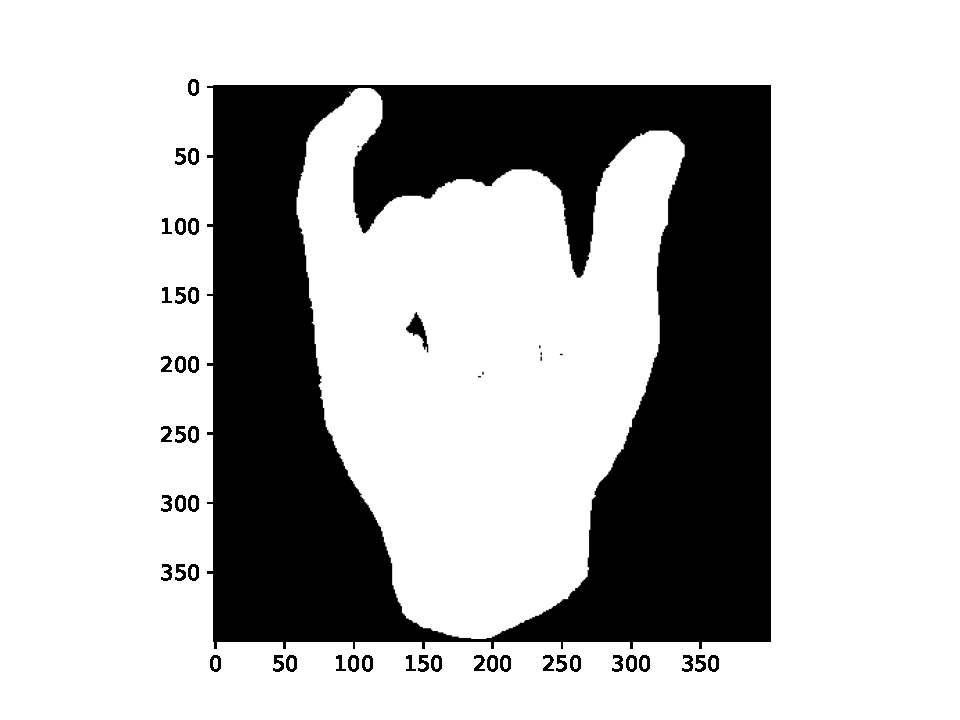
\includegraphics[width=0.75\columnwidth]{Mask.pdf}
		\caption{Mask of the image}
		\label{fig:mask}
	\end{figure}
    \begin{info}
        We tried other methods such as brightness threshold, gaussian blur and several others from the computer vision library. They all ended up 
        being less efficient than the one we finally used.
    \end{info}
		
\section{Feature extraction} \label{sec:table}
    \subsection{Keypoints}
    In the implementation of Bag of Visual Words there are two main steps to follow once you have your images: 
    Detecting the keypoints and extracting the descriptors.\\
    
    We used the SIFT algorithm to detect the keypoints
    in the image. This algorithm is one of the most implemented in the field of computer vision because of how 
    robust it is. We first tried to use \verb|detectandcompute()| (see \ref{fig:figa}) but this created a huge problem,
    when taking the background into consideration. This process is non-positional, it does not matter 
    it finds a hole in the middle of the image, (see \ref{fig:figb}), it will be treated the same as a space in the left.\\

    \begin{figure*}[b] % t for position at the top of the current page; b for position at the bottom; p for new page
		\centering
		\begin{subfigure}[b]{0.2\linewidth} % Fig (a)
			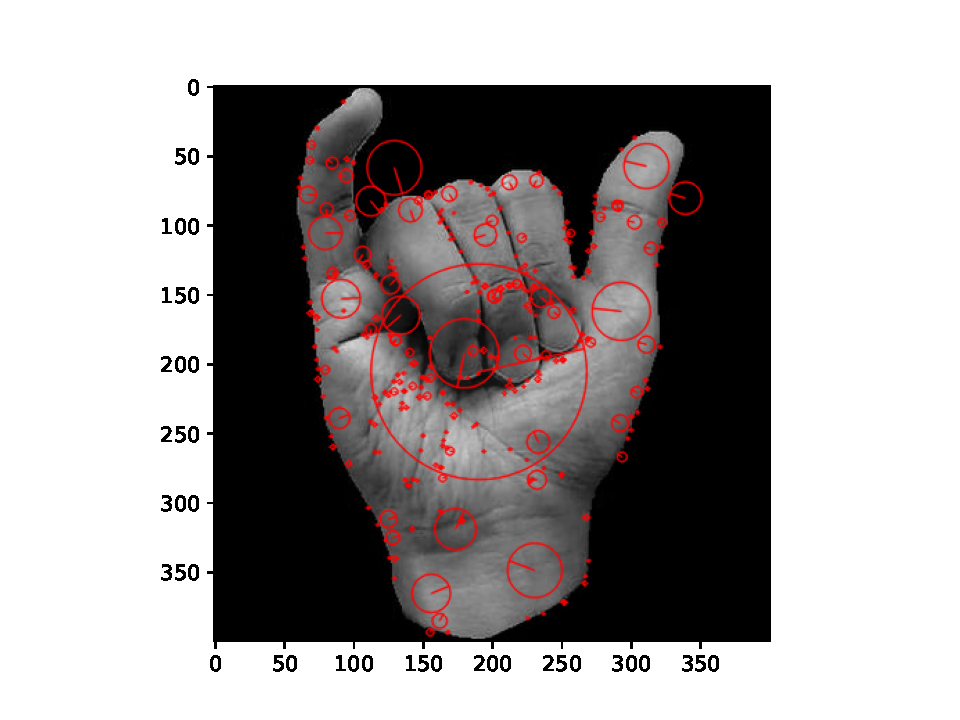
\includegraphics[width=\linewidth]{Simple_sift.pdf} % TODO: Quizá es mejor en PDF
			\caption{Simple detect and compute}
			\label{fig:figa}
		\end{subfigure}
			\hspace{20pt}   % Space between the figures
		\begin{subfigure}[b]{0.2\linewidth} % Fig (b)
			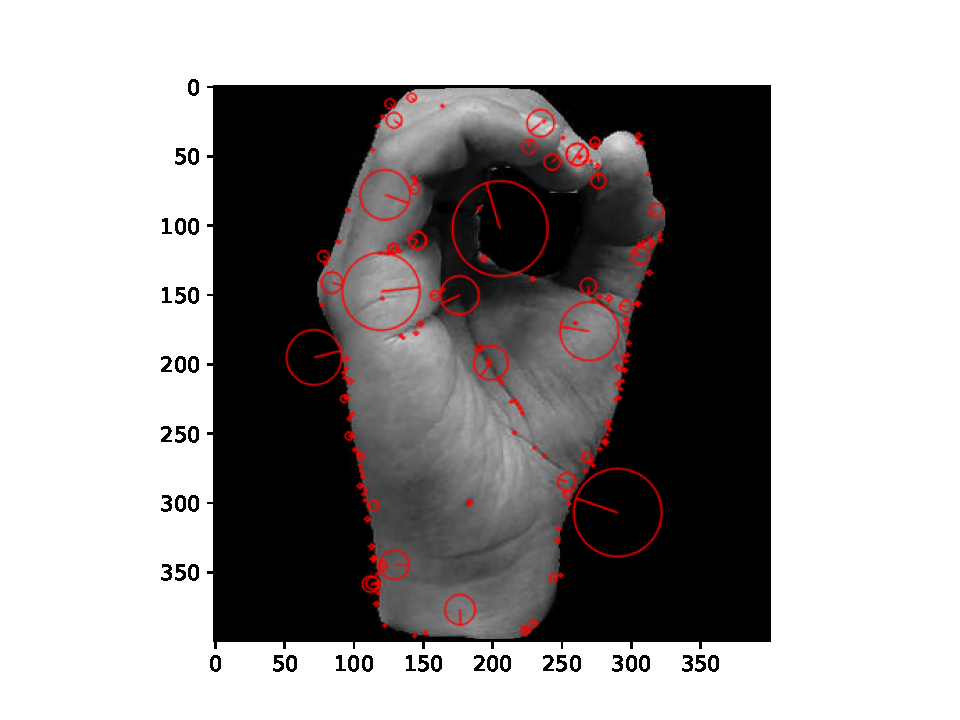
\includegraphics[width=\linewidth]{Simple_sift_mistake.pdf}
			\caption{Background mistaken keypoints}
			\label{fig:figb}
		\end{subfigure}
            \hspace{20pt} 
        \begin{subfigure}[b]{0.2\linewidth} % Fig (c)
            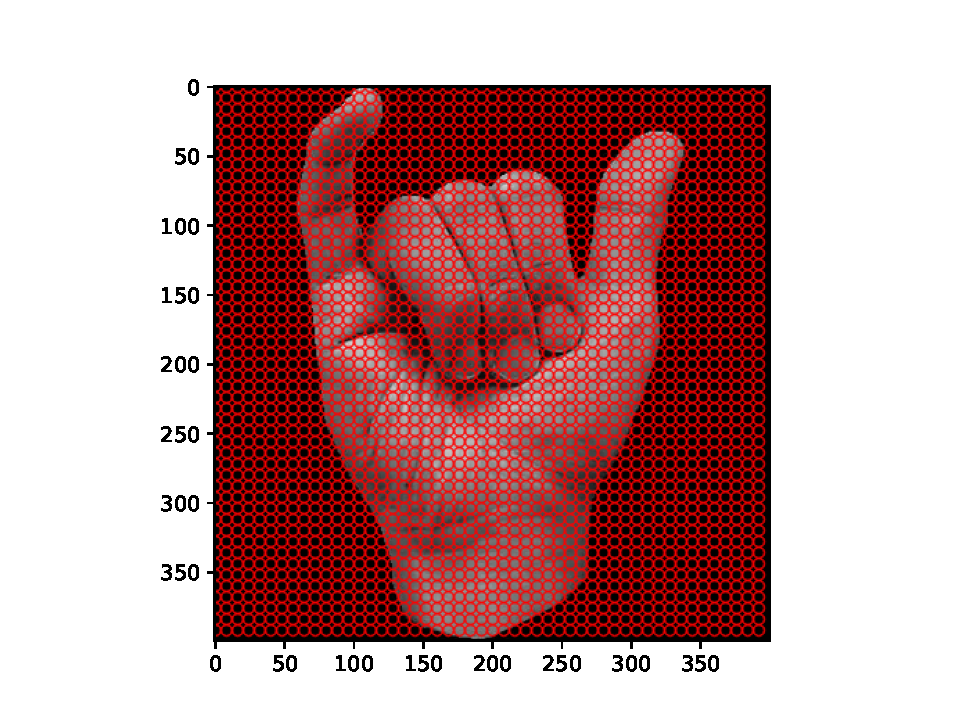
\includegraphics[width=\linewidth]{Dense_sift.pdf}
            \caption{Dense SIFT}
            \label{fig:figc}            
        \end{subfigure}
		\caption{Several keypoints detection methods considered}
		\label{fig:examplefloat}
	\end{figure*}
    After this first approach
    we tried to implement \textbf{Dense SIFT} (\ref{fig:figc}), which improved the results considerably (increasing the final accuracy by almost 15\%) but in the end 
    the game changer % TODO: muy informal?
    was the mask we applied in the previous chapter. This allowed us to remove the background and focus 
    on the hand, which allowed us to detect only the keypoints we were most interested in.

    \begin{figure}[H]
		\centering
		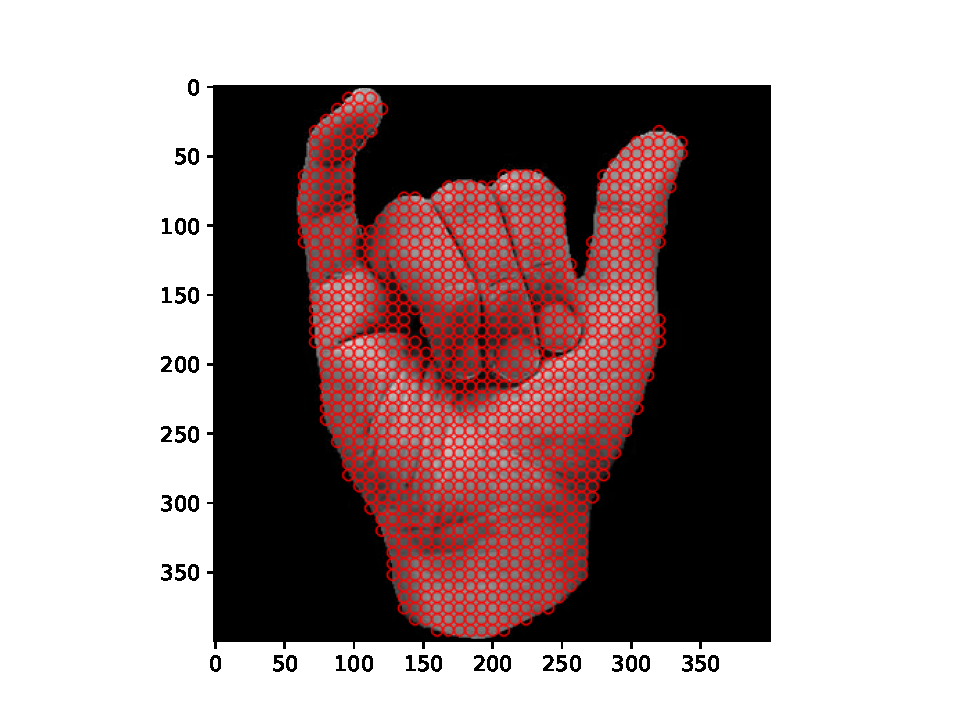
\includegraphics[width=0.75\columnwidth]{Masked_dense_sift.pdf}
		\caption{Mask applied Dense SIFT}
		\label{fig:finalsift}
	\end{figure}

    \subsection{The Codebook}

    Once we have all the descriptors from our images, we can create a codebook. The idea behind this process is to create a
    "dictionary of visual words" that will represent the most common features in our dataset. This will help us find the meaning
    behind the keypoints we have detected.\\

    In order to achieve this we implemented the KMeans algorithm. This will group all the descriptors found into 200 clusters
    which will define our codebook. This will later be used to create the histograms that will represent our images in the prediction step.


    \begin{info}
        The first number of clusters used was 36, which is the number of classes in the dataset. This was a mistake, as the codebook was not able to differentiate between the different classes. We then tried with increasing the number of clusters, which gave much better results.
    \end{info}

%    \subsection{Tables}
%	
%        Table \ref{tab:table} shows an example table. The \verb|\tabletext{}| is used to add notes to tables easily. 
%
%        \begin{info}
%        	This template uses the \texttt{booktabs} package by default. This package makes typesetting nice tables easier, but it imposes some general design guidelines. The most prominent is the distinction between middle and edge rules (horizontal lines) and the discouragement of vertical lines.
%        \end{info}
%
%        \begin{info}
%        	You should \textbf{always} avoid typesetting tables by hand. Use tools such as \href{https://www.tablesgenerator.com/}{this one} to spare yourself some unnecessary pain.
%        \end{info}
%		
%	\begin{table}[H]
%		\centering
%		\caption{Small example table.}
%		\label{tab:table}
%		\begin{tabular}{cc}
%			\toprule
%			\textbf{Column 1} & \textbf{Column 2} \\
%			\midrule
%			Data 1 & Data 2 \\
%			Data 3 & Data 4 \\
%			\bottomrule
%		\end{tabular}
%			
%            \tabletext{Note: I'm a table text for additional information.}
%			
%	\end{table}
%
\section{Predicting using the codebook}

    \subsection{From Descriptors to Histograms}
        Using the KMeans algorithm mentioned before, we can convert each image into an histogram using the codebook.
        To do this we will predict to which cluster each descriptor belongs to and then we will count how many descriptors 
        belong to each of them.

        The main objective of this process is to predict which class the image belongs by its histogram based on the fact that similar images will
        present similar histograms.

        \begin{figure*}[t] % t for position at the top of the current page; b for position at the bottom; p for new page
            \centering
            \begin{subfigure}[b]{0.2\linewidth} % Fig (a)
                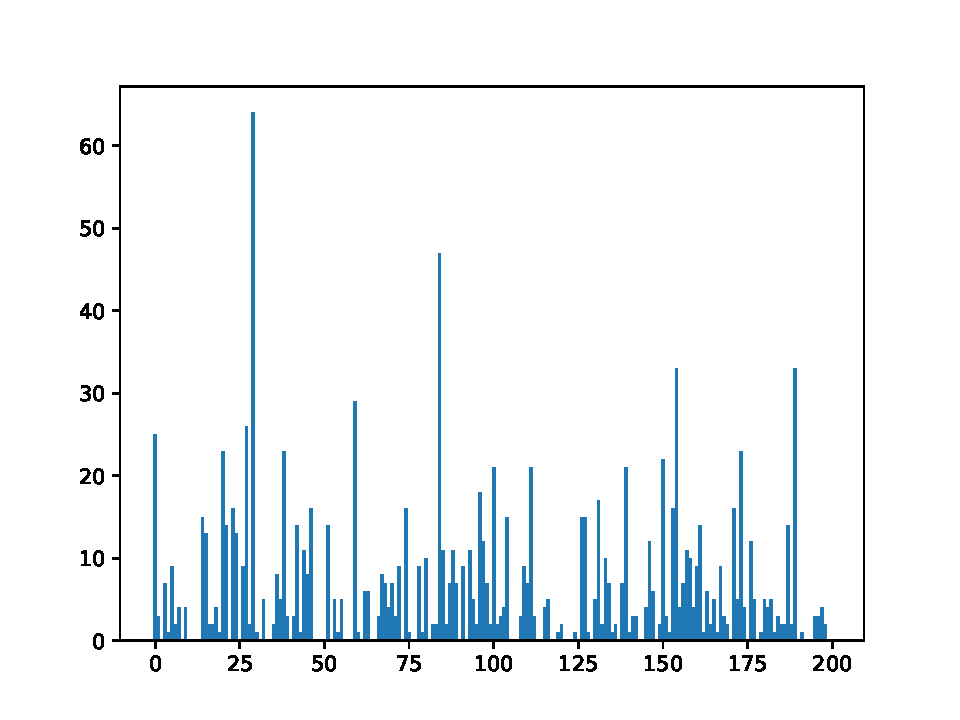
\includegraphics[width=\linewidth]{histogram0.pdf} % TODO: Quizá es mejor en PDF
                \caption{Histogram of the letter a}
                \label{fig:hista}
            \end{subfigure}
                \hspace{20pt}   % Space between the figures
            \begin{subfigure}[b]{0.2\linewidth} % Fig (b)
                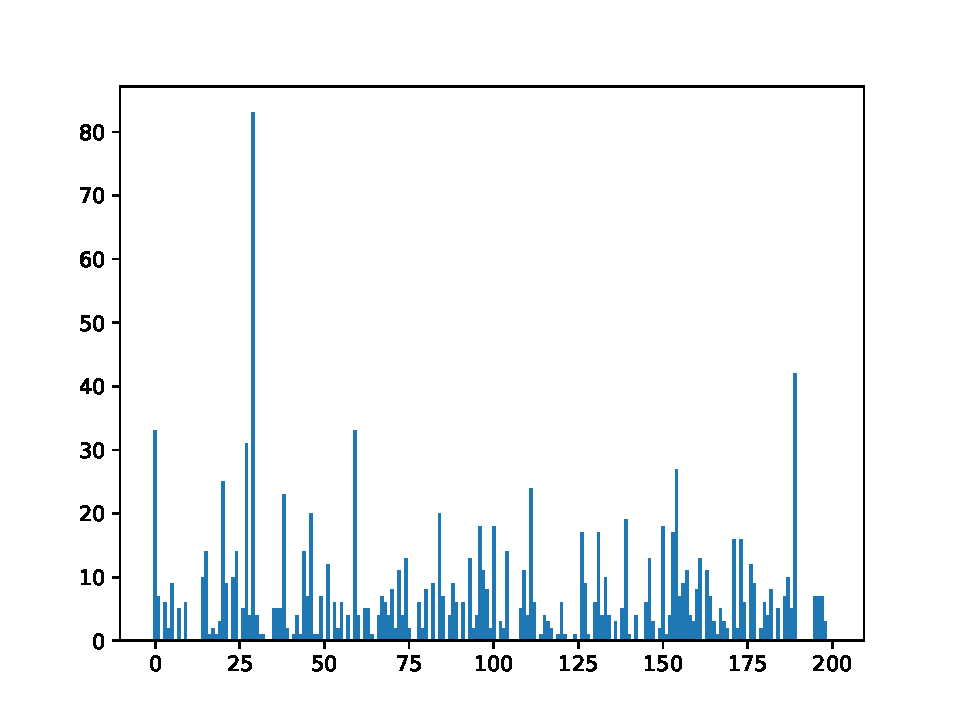
\includegraphics[width=\linewidth]{histogram1.pdf}
                \caption{Histogram of a different photo of the letter a}
                \label{fig:histb}
            \end{subfigure}
                \hspace{20pt} 
            \begin{subfigure}[b]{0.2\linewidth} % Fig (c)
                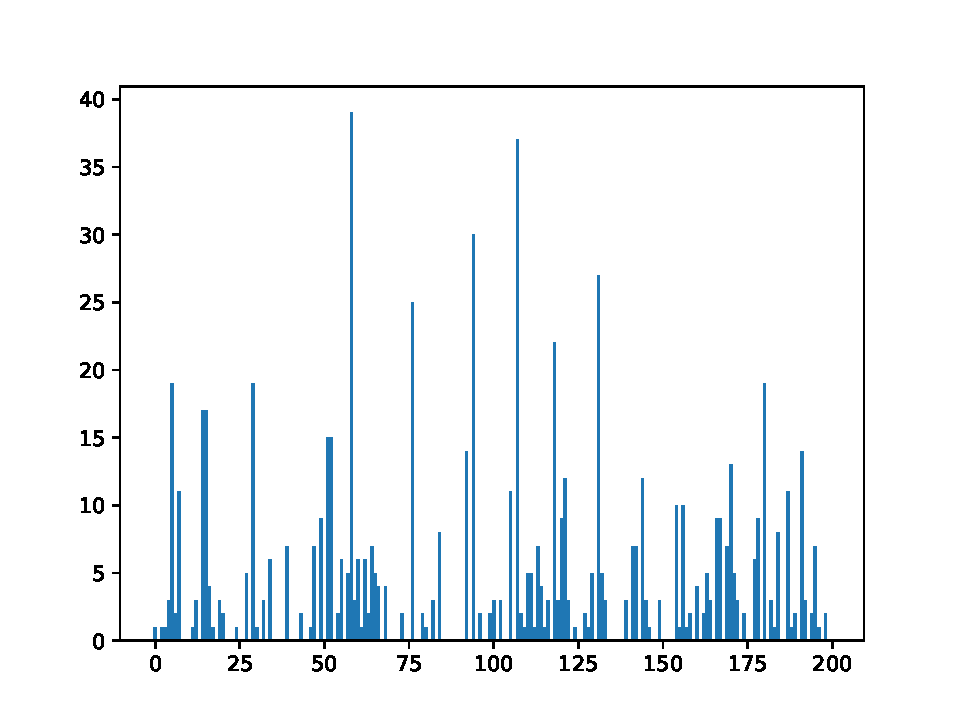
\includegraphics[width=\linewidth]{histogram2.pdf}
                \caption{Histogram of the letter p}
                \label{fig:histc}            
            \end{subfigure}
            \caption{Comparison of histograms of different images}
            \label{fig:histograms}
        \end{figure*}
		
	We can observe in Figure \ref{fig:histograms} that the first two histograms, corresponding to two different images categorised as the letter "a", are very similar.
    The main features (the peaks) are in the same position, while the histogram of the letter "p" is completely different. This is the main idea behind the idea of the codebook.
    
    \subsection{SVM}
        There are lots of different models that can be used to predict the categories of these histograms, the one we ended up choosing is SVM
        (Support Vector Machines). After doing a split between the train and the test we tried a starting model with a linear kernel. After 
        this first approach, we tried to improve the model by using a grid search to find the best hyperparameters. After looking at the classification reports, this are the results:\\

        \begin{tabular}{c | c c c}
            \centering
            & Precision & Recall & F1-score \\
            \hline
            Simple model & 0.96 & 0.96 & 0.96 \\
            Grid search & 0.97 & 0.97 & 0.97 \\
        \end{tabular}\\
		
        Once we have the complete process, we compressed all the operations in one unique function \verb|predict_image|
        \nolinenumbers
            \lstinputlisting[caption=Predict Image Function., language=Python,label=code]{func.py}
	    \linenumbers
\section{Video Processing}
        
        Now we have a model that can correctly predict the category of an image. We can use this model to predict the category of each frame of a video\footnote{The video used corresponds to \href{https://www.youtube.com/watch?v=FK1aj2Aw1Mg}{ASL Fingerspelling Exercise} from \textit{Learn How to Sign}}.
        To do this we will use the \verb|cv2.VideoCapture()| function together with a ratio variable to take 1 of every few frames. This will allow us to
        process the video faster and will help us to avoid the transition frames between signs.\\

        \begin{figure}[H]
            \centering
            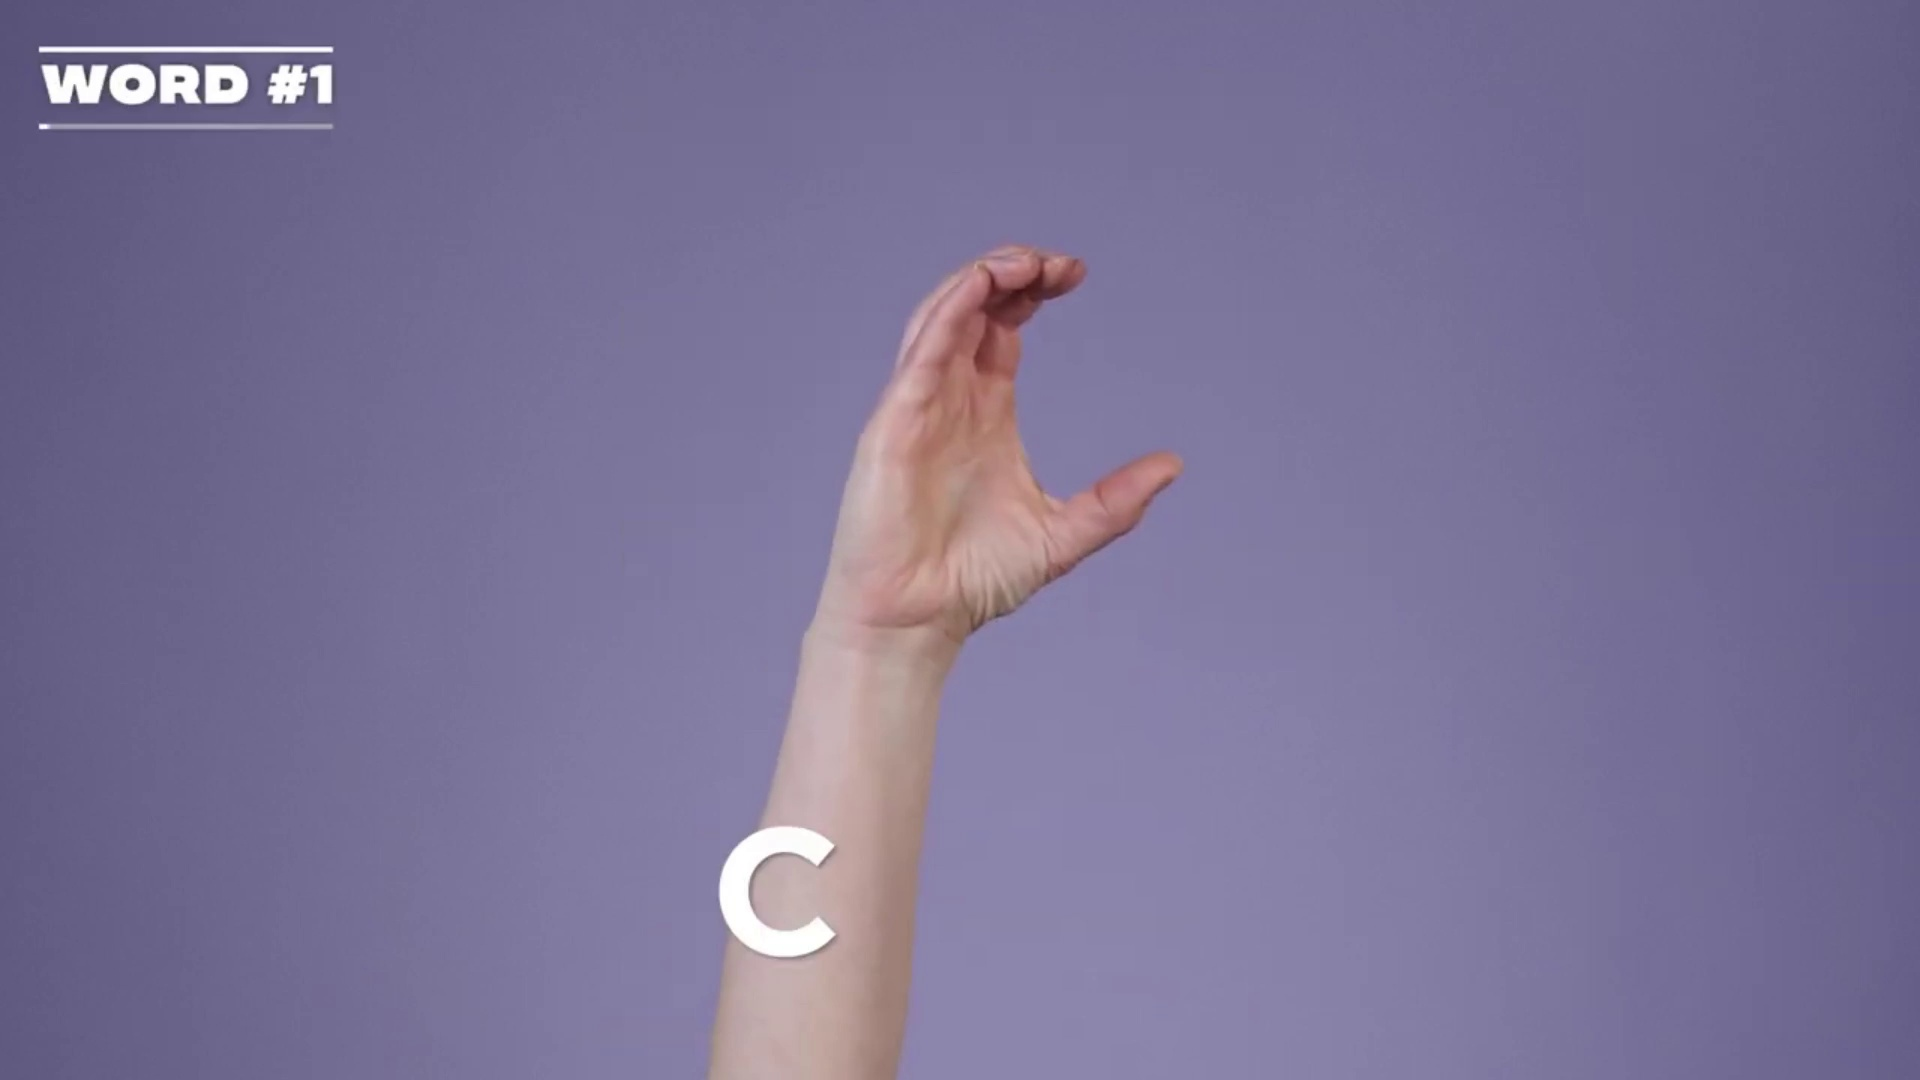
\includegraphics[width=0.75\columnwidth]{frame40.jpg}
            \caption{Frame of the spelling video}
            \label{fig:Frame}
        \end{figure}

        Once we have extracted some frames from the video, we need to process it into images we can predict.
\section{Hand Detection}
	As it seems, there is a lot of noise in the frames extracted (text, coloured background, etc.). In order to have a better accuracy when predicting the ASL symbols, we first need to detect the hand in the frame.\\

    To do this we used the \verb|hands| library from \verb|MediaPipe| in order to detect the hand in the frame.
    \begin{figure}[H]
        \centering
        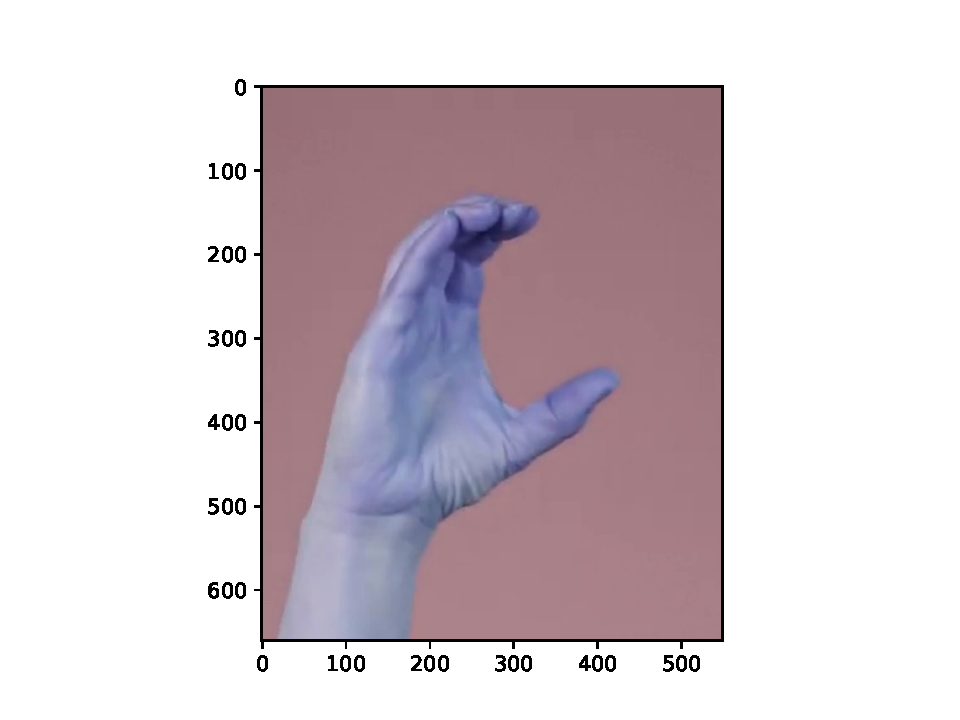
\includegraphics[width=0.75\columnwidth]{cropped_frame.pdf}
        \caption{Hand detected in the frame}
        \label{fig:crop_frame}
    \end{figure}

    Once we have the cropped image we apply the same mask as before to remove the background and focus on the hand, in order to predict the result with better accuracy.
    \begin{figure}[H]
        \centering
        \begin{subfigure}[b]{0.43\linewidth}
            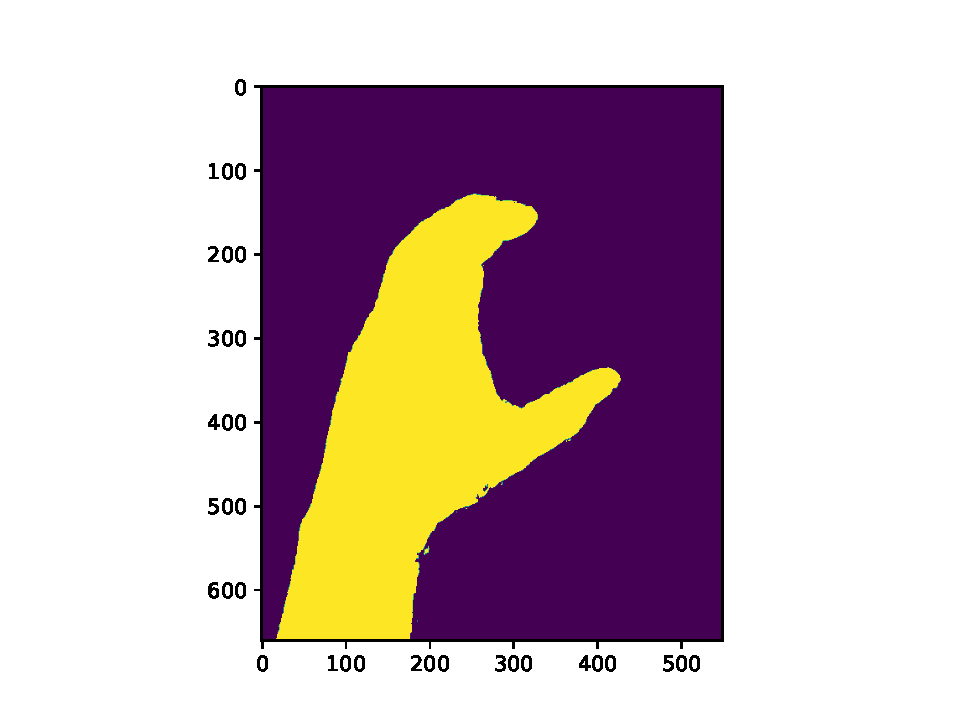
\includegraphics[width=\linewidth]{cropped_mask.pdf}
            \caption{Mask applied to the cropped image}
            \label{fig:crop_mask}
        \end{subfigure}
        \hspace{2pt}
        \begin{subfigure}[b]{0.43\linewidth}
            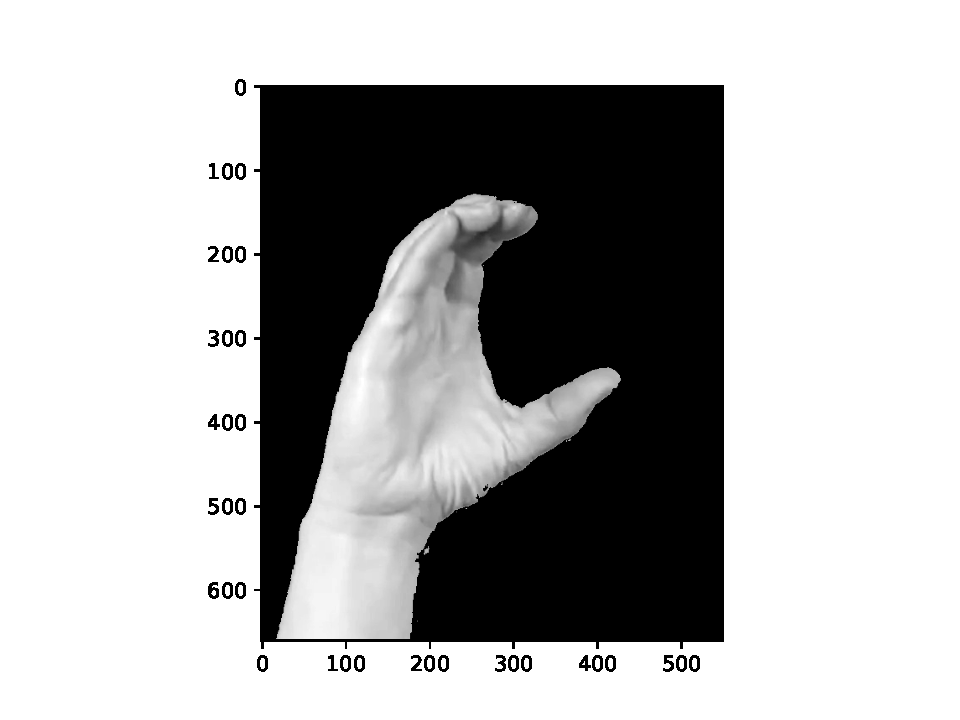
\includegraphics[width=\linewidth]{cropped_result.pdf}
            \caption{Result after applying the mask}
            \label{fig:crop_res}
        \end{subfigure}
        \caption{Applying the mask to the cropped image}
    \end{figure}

    Once we have removed the background, just as way to standarize our photos, the images will be resized into 400x400px, the size of the dataset images.
    \begin{figure}[H]
        \centering
        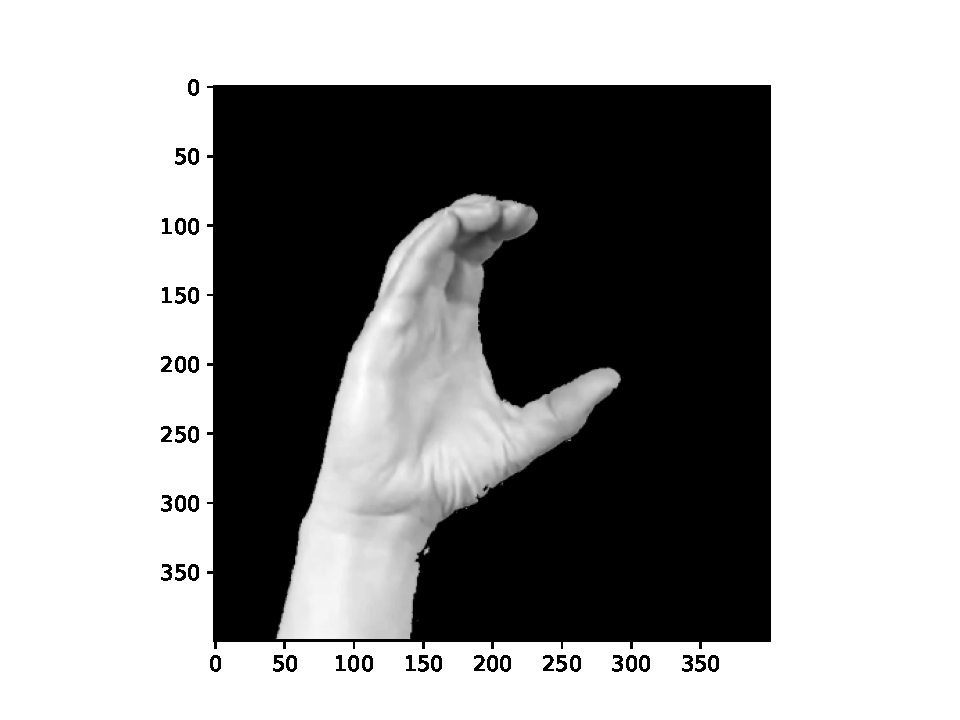
\includegraphics[width=0.75\columnwidth]{cropped_resized.pdf}
        \caption{Final preprocessed hand}
    \end{figure}
\section{Final Results}
    After doing a prediction of all the images the results presented some problems. One of the main ones was the transition and "no sign" frames that appeared between the different signs.
    This derived in a lot of noise in the final prediction. In order to adjust this, one solution was to adjust the ratio of frames, or take a majority voting of several sections of the prediction.\\

    However, a second problem appeared. Some signs, such as the "A" and the "T" or the "I" and the "J" are really similar which created confusion in the prediction on the model.\\

    The predictor is able to detect and classify particularly selected frames, nevertheless, the solution to the noise and confusion problems is still under development.
    Here are some of the results of the prediction (see Figure \ref{fig:preds}).
    \begin{figure*}[b] % t for position at the top of the current page; b for position at the bottom; p for new page
        \centering
        \begin{subfigure}[b]{0.2\linewidth} % Fig (a)
            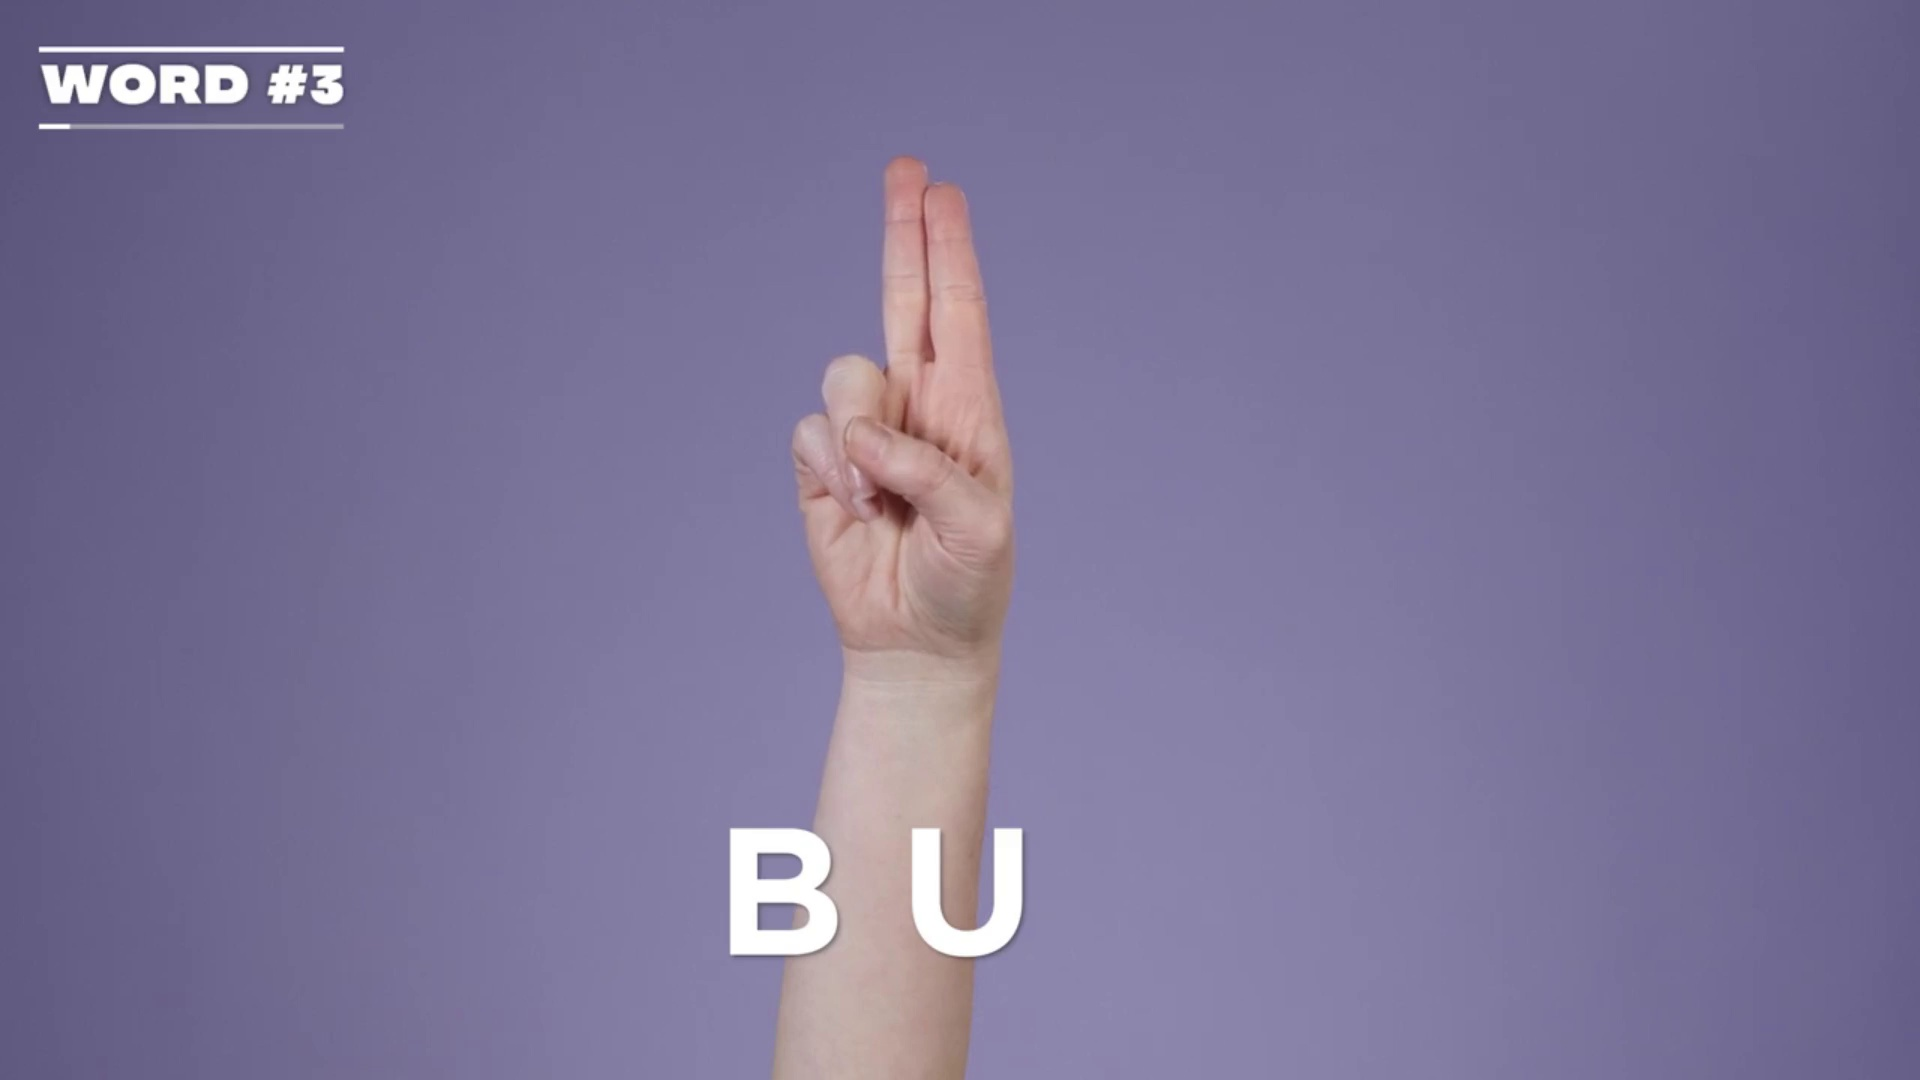
\includegraphics[width=\linewidth]{frame64.jpg} % TODO: Quizá es mejor en PDF
            \caption{Original frame of the letter U}
            \label{fig:frameu}
        \end{subfigure}
            \hspace{20pt}   % Space between the figures
        \begin{subfigure}[b]{0.2\linewidth} % Fig (b)
            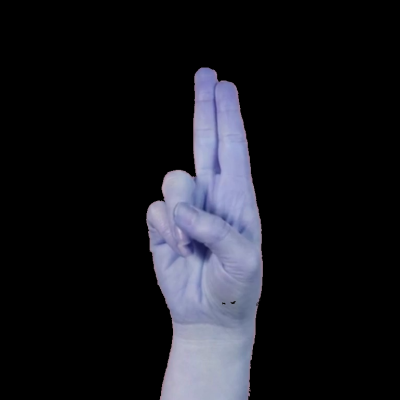
\includegraphics[width=\linewidth]{frame64.jpg_processed.png}
            \caption{Processed frame predicted as "U"}
            \label{fig:predu}
        \end{subfigure}
            \hspace{20pt}
        \begin{subfigure}[b]{0.2\linewidth} % Fig (a)
            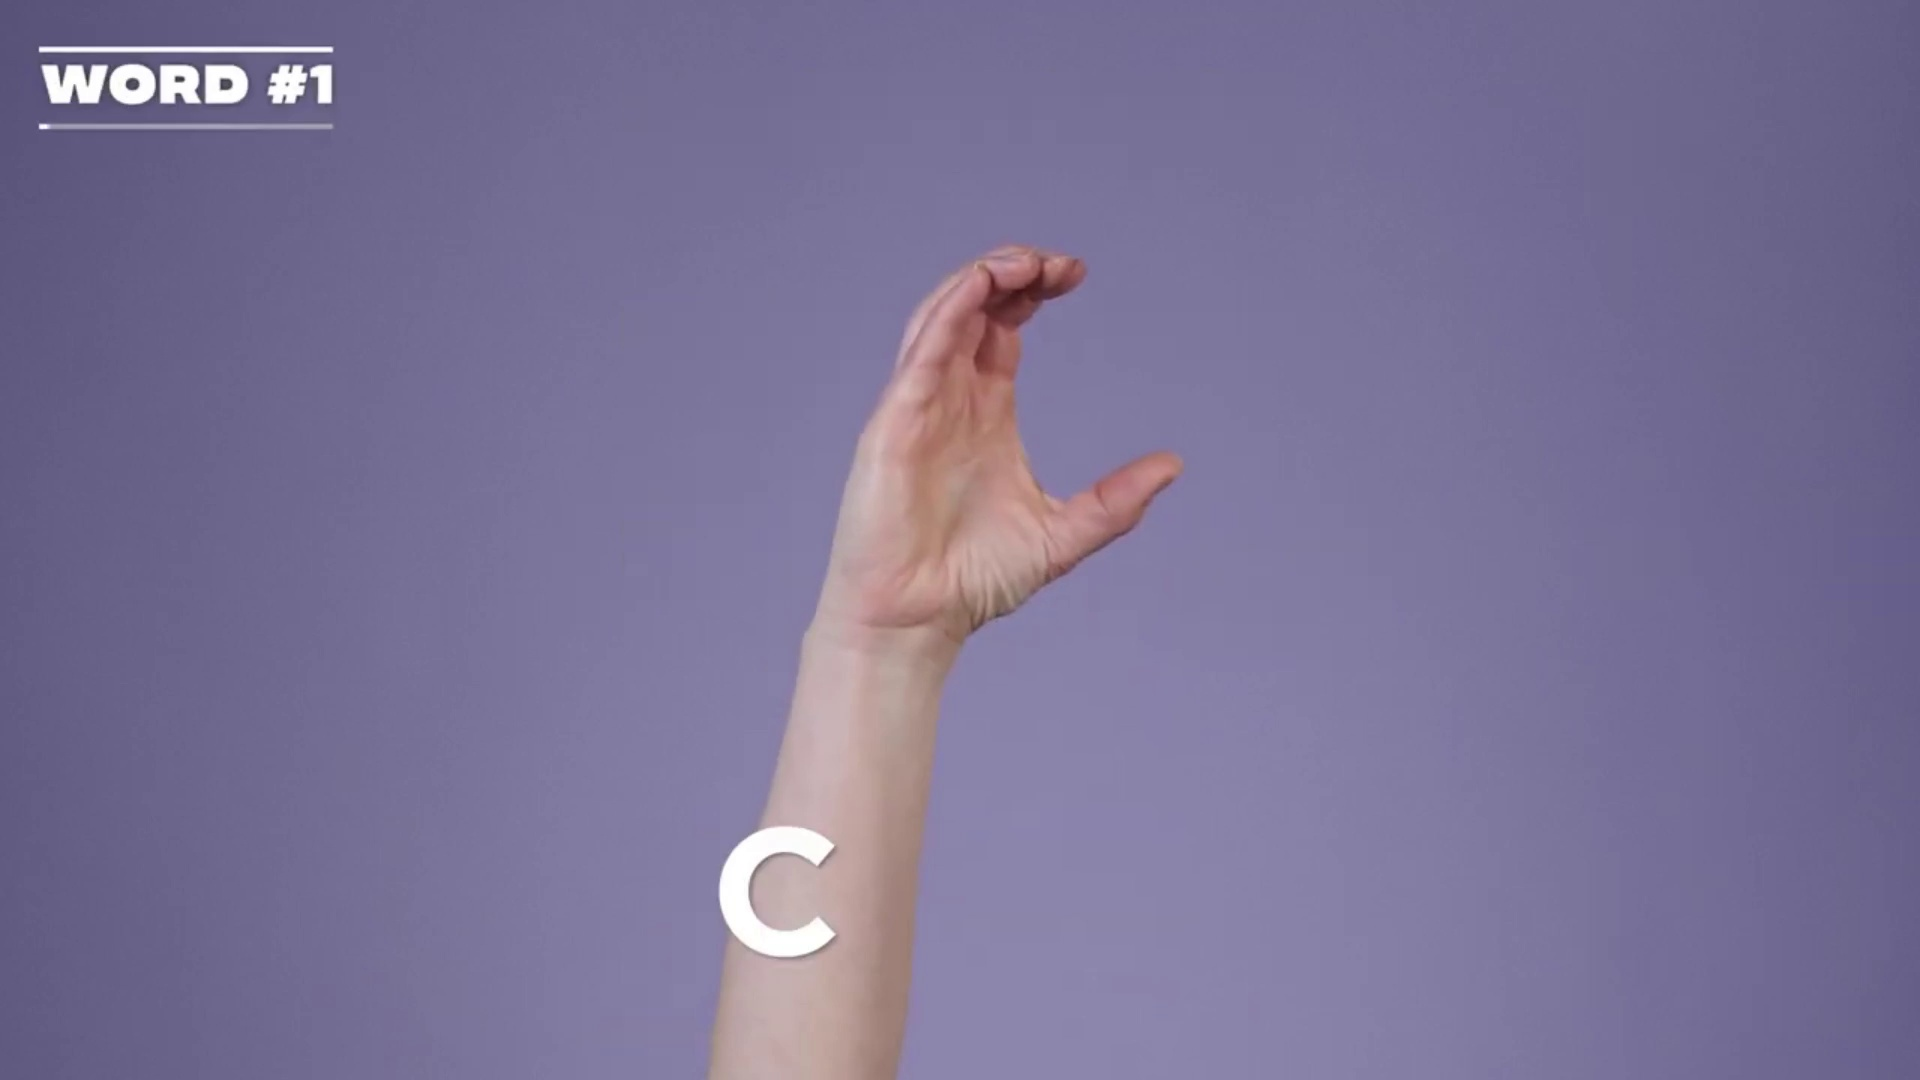
\includegraphics[width=\linewidth]{frame40.jpg} % TODO: Quizá es mejor en PDF
            \caption{Original frame of the letter C}
            \label{fig:framec}
        \end{subfigure}
            \hspace{20pt}   % Space between the figures
        \begin{subfigure}[b]{0.2\linewidth} % Fig (b)
            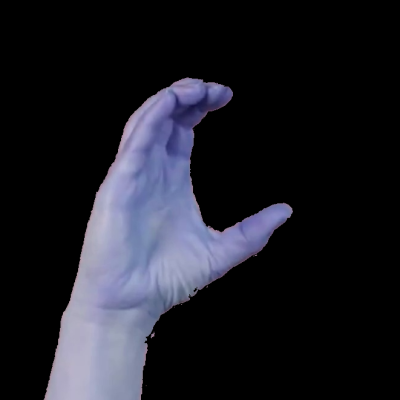
\includegraphics[width=\linewidth]{frame40.jpg_processed.png}
            \caption{Processed frame predicted as "C"}
            \label{fig:predc}
        \end{subfigure}
        
        \caption{Image predictions of the video}
        \label{fig:preds}
    \end{figure*}
    

	
\section{Future Improvements}
    \subsection{Category Coherence}
        One of the main problems we have found when predicting is the different ways that exist to sign the same letter. This is a problem that can be solved by adding more variability to the images that train the model. We can appreciate this problem if we compare the letter "G" in the video and the dataset.
    \subsection{Transition Frames}
        The problem with the transition frames has many solutions, but none of them has ended working for the purpouse of the project. A future upgrade to the frame extraction step will be selecting only the frames that present a really small variance with the previous one.
        The idea behind this solution is to have into account that when signing, the hand will not move a lot between the frames corresponding to the same letter.
    \subsection{Model Improvement}
        The model can be improve by fine tuning the model even more or trying different classifiers. The solution we have in mind is implementing a Neural Network to predict the sign, but that solution will be applied in future approaches to this problem.

%----------------------------------------------------------

%\addcontentsline{toc}{section}{References}
%\printbibliography

%----------------------------------------------------------

\end{document}